% !TeX document-id = {e8a7e607-95aa-4aa4-a520-082b73312f40}
% !TeX spellcheck = de_DE
% !TeX TXS-program:compile = txs:///pdflatex/[--shell-escape]

%----------------------------------------------------------------------------------------
%       PACKAGES AND OTHER DOCUMENT CONFIGURATIONS
%----------------------------------------------------------------------------------------
\documentclass[paper=a4, fontsize=12pt]{article}
\usepackage[german]{babel} % English language/hyphenation
\usepackage{amsmath,amsfonts,amsthm,mathtools} % Math packages
\usepackage[utf8]{inputenc}
\usepackage{float}
\usepackage{lipsum} % Package to generate dummy text throughout this template
\usepackage{blindtext}
\usepackage{graphicx} 
\usepackage{caption}
\usepackage{subcaption}
\usepackage[sc]{mathpazo} % Use the Palatino font
\usepackage[T1]{fontenc} % Use 8-bit encoding that has 256 glyphs
\linespread{1.05} % Line spacing - Palatino needs more space between lines
\usepackage{microtype} % Slightly tweak font spacing for aesthetics
\usepackage[hmarginratio=1:1,top=32mm,left=2cm,right=1cm ,columnsep=20pt]{geometry} % Document margins
%\usepackage[hang, small,labelfont=bf,up,textfont=it,up]{caption} % Custom captions under/above floats in tables or figures
\usepackage[hidelinks]{hyperref} % For hyperlinks in the PDF
\usepackage{lettrine} % The lettrine is the first enlarged letter at the beginning of the text
\usepackage{paralist} % Used for the compactitem environment which makes bullet points with less space between them
\usepackage{abstract} % Allows abstract customization
\renewcommand{\abstractnamefont}{\normalfont\bfseries} % Set the "Abstract" text to bold
\renewcommand{\abstracttextfont}{\normalfont\small\itshape} % Set the abstract itself to small italic text
\usepackage{titlesec} % Allows customization of titles
\setlength{\parindent}{0pt}

\renewcommand\thesection{\Roman{section}} % Roman numerals for the sections
\renewcommand\thesubsection{\Roman{subsection}} % Roman numerals for subsections

\titleformat{\section}[block]{\large\scshape\centering}{\thesection.}{1em}{} % Change the look of the section titles
\titleformat{\subsection}[block]{\large}{\thesubsection.}{1em}{} % Change the look of the section titles
\newcommand{\horrule}[1]{\rule{\linewidth}{#1}} % Create horizontal rule command with 1 argument of height
\usepackage{fancyhdr} % Headers and footers
\pagestyle{fancy} % All pages have headers and footers
\fancyhead{} % Blank out the default header
\fancyfoot{} % Blank out the default footer

\fancyhead[C]{Hamburg University of Applied Sciences $\,\bullet\,$ BTI4-RNP/02} % Custom header text

\fancyfoot[RO,LE]{\thepage} % Custom footer text


%----------------------------------------------------------------------------------------
%       SYNTAX HIGHLIGHTING
%
% Show available Languages: pygmentize -L
%----------------------------------------------------------------------------------------
\usepackage{minted}

\newminted{java}{autogobble, tabsize = 2, frame=single, breaklines, fontfamily=courier, fontsize=\footnotesize}
\newmintinline{java}{autogobble, fontfamily=courier, style=bw}

\newminted{c}{autogobble, tabsize = 2, frame=single, breaklines, fontfamily=courier, fontsize=\footnotesize}
\newmintinline{c}{autogobble, fontfamily=courier, style=bw}

\newminted{cpp}{autogobble, tabsize = 2, frame=single, breaklines, fontfamily=courier, fontsize=\footnotesize}
\newmintinline{cpp}{autogobble, fontfamily=courier, style=bw}

\newminted{php}{autogobble, tabsize = 2, frame=single, breaklines, fontfamily=courier, fontsize=\footnotesize}
\newmintinline{php}{autogobble, fontfamily=courier, style=bw}

\newminted{text}{autogobble,tabsize = 2, frame=single, breaklines, fontfamily=courier, fontsize=\footnotesize}
\newmintinline{text}{fontfamily=courier, style=bw}

\newminted{bash}{autogobble, tabsize = 2, frame=single, breaklines, fontfamily=courier, fontsize=\footnotesize}
\newmintinline{bash}{autogobble, fontfamily=courier, style=bw}

\newminted{matlab}{autogobble, tabsize = 2, frame=single, breaklines, fontfamily=courier, fontsize=\footnotesize}
\newmintinline{matlab}{autogobble, fontfamily=courier, style=bw}

%----------------------------------------------------------------------------------------
%       TITLE SECTION
%----------------------------------------------------------------------------------------
\title{\vspace{-15mm}\fontsize{24pt}{10pt}\selectfont\textbf{Entwurfsdokument}} % Article title
\author{
    \large
    {\textsc{Praktikum 2 Threads}}\\[2mm]
    {\textsc{Hauke Goldhammer (2286057)}}\\[2mm]
    {\textsc{Martin Witte (2285586)}}\\[2mm]
    %\thanks{A thank you or further information}\\ % Your name
    %\normalsize \href{mailto:marco.torres.810@gmail.com}{marco.torres.810@gmail.com}\\[2mm] % Your email address
}
%\date{} % Uncomment to remove date

%----------------------------------------------------------------------------------------
\begin{document}
\maketitle % Insert title
\thispagestyle{fancy} % All pages have headers and footers

\section{Aufgabenstellung:}
Zu erstellen ist ein Programm, mit folgenden Anforderungen:\\
- Einen Mainthread hat, welcher die anderen Threads startet und wartet, bis alle anderen Threads fertig sind.\\
- Einen Producer\_ 1 Thread, der a, b,..., y, z ; in einen Puffer schreibt und ausgibt, was er getan hat. Er blockiert wenn der Puffer voll ist und schreibt weiter, wenn wieder Platz ist.\\
- Einen Producer\_ 2 Thread, wie Producer\_ 1, aber Großbuchstaben.\\
- Einen Consumer Thread, welcher alle 2 Sekunden ein Zeichen aus dem Puffer nimmt und dieses ausgibt. Wenn der Puffer leer ist blockiert der Thread, bis wieder Zeichen im Puuer sind.\\
- Einen Control Thread, dieser soll mit Tastatureingaben, dass System steuern.

\subsection{Bedienungsanforderungen:}
\subsubsection{Tastatureingaben:}
- '1' $\rightarrow$ Start/Stopp Producer\_ 1\\
- '2' $\rightarrow$ Start/Stopp Producer\_ 2\\
- 'c' oder 'C' $\rightarrow$ Start/Stopp Consumer\\
- 'q' oder 'Q' $\rightarrow$ Main-Thread beendet das System\\
- 'h' $\rightarrow$ hilfe\\

\subsection{Weitere Anforderungen:}
\begin{tabular}{l|l}
Anforderung & Lösungsansatz \\
\hline
Wahl zwischen den 2 Varianten &  args bei Programmstart(s, c), dann arbeitet das Prog \\
  & entweder mit Queue\_ sema oder Queue\_ condi\\
\hline
Kein Polling & zum blockieren mutex nutzen \\ 
\hline
Angehaltene Threads müssen blockiert werden & mutex nutzen \\ 
\hline
FIFU\_ 1 mit Semaphoren &  \\ 
\hline
FIFU\_ 2 mit Conditional Variables & \\
\hline
Makefile erstellen &  \\
\hline
Fehlermeldungen gem. POSIX bzw. errno &  \\
\hline
Beenden von Threads nicht in kritischen Abschnitten & //Zwei Möglichkeiten!! \\
\hline
Mutexe+Semaphore am Ende wieder an BS zurückgeben & destroy-Funktionen (vorher unlock beachten) \\
\hline
Funktionen möglichst generisch &  \\
\end{tabular}
\\
\\
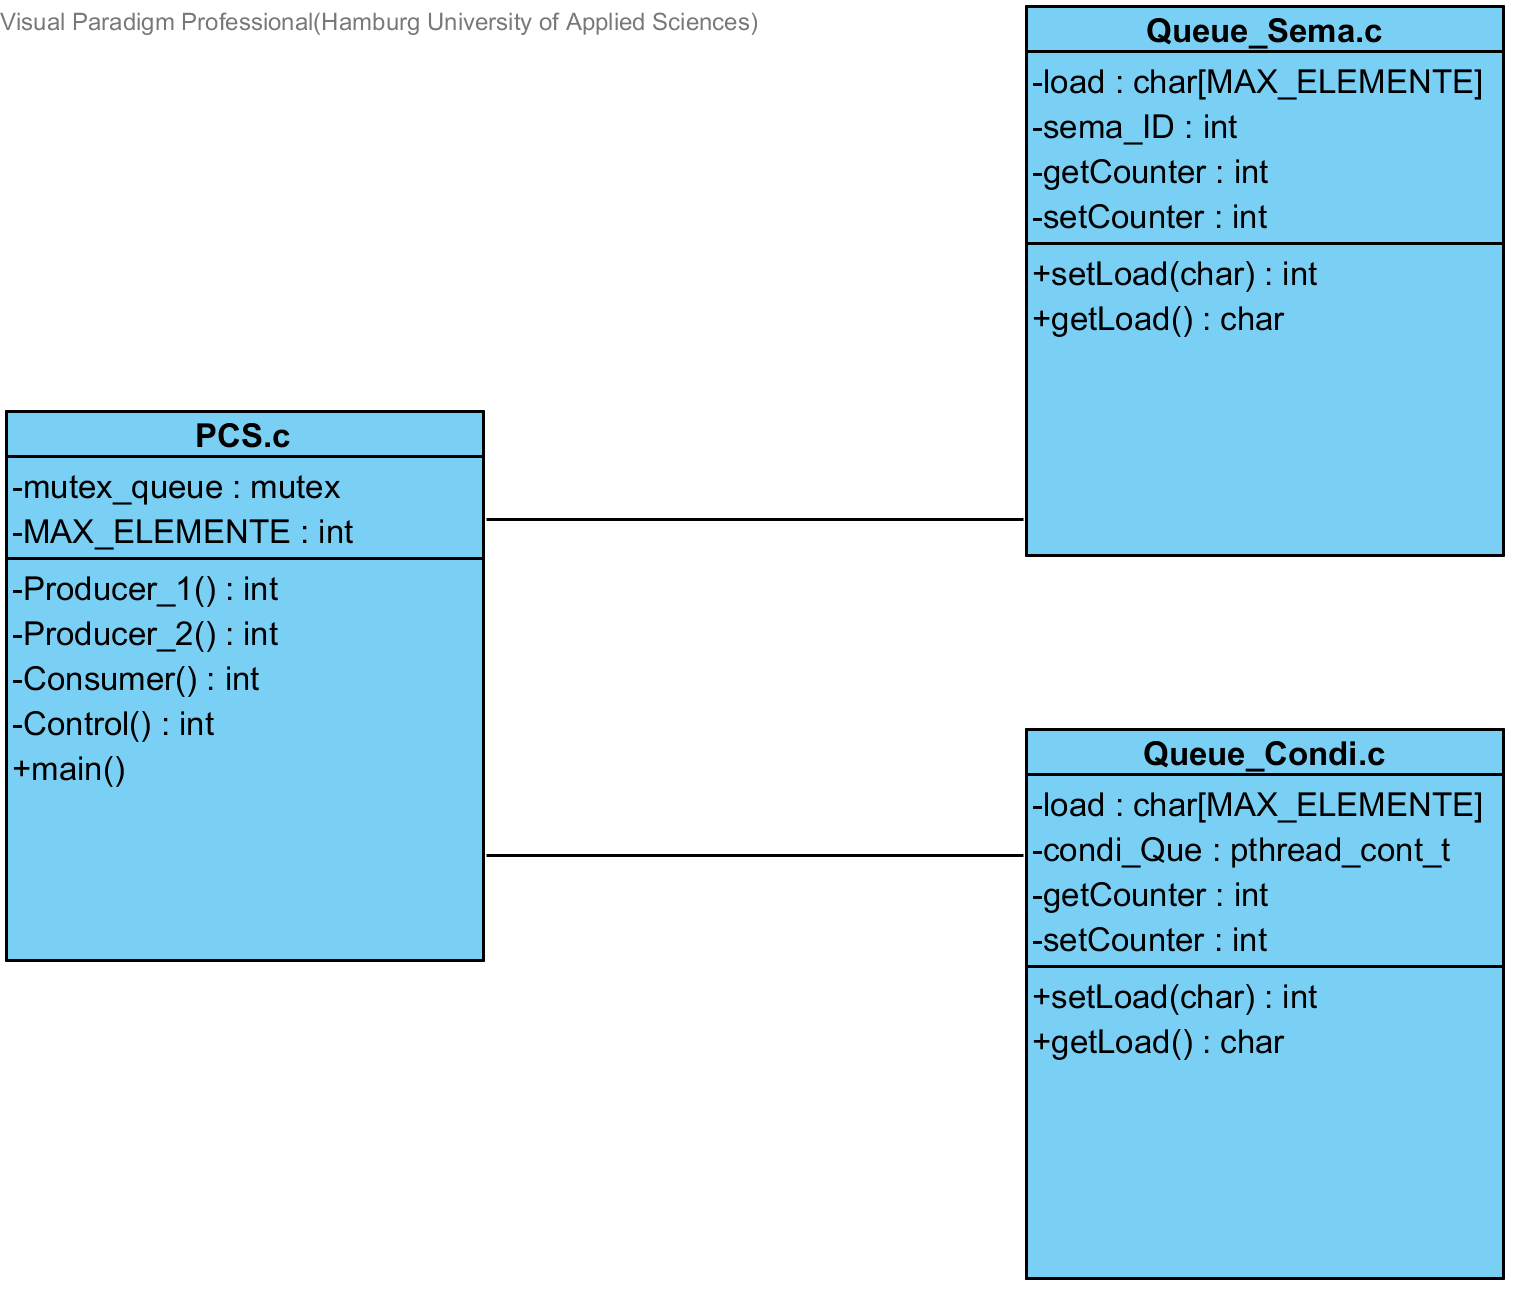
\includegraphics[scale=1]{Entwurf v1-0.png}

\end{document}